
%% bare_jrnl_compsoc.tex
%% V1.4b
%% 2015/08/26
%% by Michael Shell
%% See:
%% http://www.michaelshell.org/
%% for current contact information.
%%
%% This is a skeleton file demonstrating the use of IEEEtran.cls
%% (requires IEEEtran.cls version 1.8b or later) with an IEEE
%% Computer Society journal paper.
%%
%% Support sites:
%% http://www.michaelshell.org/tex/ieeetran/
%% http://www.ctan.org/pkg/ieeetran
%% and
%% http://www.ieee.org/

%%*************************************************************************
%% Legal Notice:
%% This code is offered as-is without any warranty either expressed or
%% implied; without even the implied warranty of MERCHANTABILITY or
%% FITNESS FOR A PARTICULAR PURPOSE! 
%% User assumes all risk.
%% In no event shall the IEEE or any contributor to this code be liable for
%% any damages or losses, including, but not limited to, incidental,
%% consequential, or any other damages, resulting from the use or misuse
%% of any information contained here.
%%
%% All comments are the opinions of their respective authors and are not
%% necessarily endorsed by the IEEE.
%%
%% This work is distributed under the LaTeX Project Public License (LPPL)
%% ( http://www.latex-project.org/ ) version 1.3, and may be freely used,
%% distributed and modified. A copy of the LPPL, version 1.3, is included
%% in the base LaTeX documentation of all distributions of LaTeX released
%% 2003/12/01 or later.
%% Retain all contribution notices and credits.
%% ** Modified files should be clearly indicated as such, including  **
%% ** renaming them and changing author support contact information. **
%%*************************************************************************


% *** Authors should verify (and, if needed, correct) their LaTeX system  ***
% *** with the testflow diagnostic prior to trusting their LaTeX platform ***
% *** with production work. The IEEE's font choices and paper sizes can   ***
% *** trigger bugs that do not appear when using other class files.       ***                          ***
% The testflow support page is at:
% http://www.michaelshell.org/tex/testflow/


\documentclass[10pt,journal,compsoc]{IEEEtran}
%
% If IEEEtran.cls has not been installed into the LaTeX system files,
% manually specify the path to it like:
% \documentclass[10pt,journal,compsoc]{../sty/IEEEtran}


\usepackage[T1]{fontenc}
\usepackage[utf8]{inputenc}
\usepackage[ngerman]{babel}

%% asm
\usepackage{amsmath}
\usepackage{amsfonts}
\usepackage{amssymb}

%% utilities
\usepackage{graphicx}
\usepackage{tikz}
\usepackage{multicol}
\usepackage{slashbox}
\usepackage{ntheorem}
\usepackage{listings}
\usepackage{color}

\definecolor{mygreen}{rgb}{0,0.6,0}
\definecolor{mygray}{rgb}{0.5,0.5,0.5}
\definecolor{mymauve}{rgb}{0.58,0,0.82}

\lstset{ %
  backgroundcolor=\color{white},   % choose the background color; you must add \usepackage{color} or \usepackage{xcolor}; should come as last argument
  basicstyle=\footnotesize,        % the size of the fonts that are used for the code
  breakatwhitespace=false,         % sets if automatic breaks should only happen at whitespace
  breaklines=true,                 % sets automatic line breaking
  captionpos=b,                    % sets the caption-position to bottom
  commentstyle=\color{mygreen},    % comment style
  deletekeywords={...},            % if you want to delete keywords from the given language
  escapeinside={(*}{*)},          % if you want to add LaTeX within your code
  extendedchars=true,              % lets you use non-ASCII characters; for 8-bits encodings only, does not work with UTF-8
  frame=single,	                   % adds a frame around the code
  keepspaces=true,                 % keeps spaces in text, useful for keeping indentation of code (possibly needs columns=flexible)
  keywordstyle=\color{blue},       % keyword style
  language=Python,                 % the language of the code
  morekeywords={*,...},           % if you want to add more keywords to the set
  numbers=left,                    % where to put the line-numbers; possible values are (none, left, right)
  numbersep=8pt,                   % how far the line-numbers are from the code
  numberstyle=\tiny\color{mygray}, % the style that is used for the line-numbers
  rulecolor=\color{black},         % if not set, the frame-color may be changed on line-breaks within not-black text (e.g. comments (green here))
  showspaces=false,                % show spaces everywhere adding particular underscores; it overrides 'showstringspaces'
  showstringspaces=false,          % underline spaces within strings only
  showtabs=false,                  % show tabs within strings adding particular underscores
  stepnumber=1,                    % the step between two line-numbers. If it's 1, each line will be numbered
  stringstyle=\color{mymauve},     % string literal style
  tabsize=2,	                   % sets default tabsize to 2 spaces
  title=\lstname                   % show the filename of files included with \lstinputlisting; also try caption instead of title
}

% *** CITATION PACKAGES ***
%
\ifCLASSOPTIONcompsoc
  % IEEE Computer Society needs nocompress option
  % requires cite.sty v4.0 or later (November 2003)
  \usepackage[nocompress]{cite}
\else
  % normal IEEE
  \usepackage{cite}
\fi
% *** GRAPHICS RELATED PACKAGES ***
%
\ifCLASSINFOpdf
  % \usepackage[pdftex]{graphicx}
  % declare the path(s) where your graphic files are
  % \graphicspath{{../pdf/}{../jpeg/}}
  % and their extensions so you won't have to specify these with
  % every instance of \includegraphics
  % \DeclareGraphicsExtensions{.pdf,.jpeg,.png}
\else
  % or other class option (dvipsone, dvipdf, if not using dvips). graphicx
  % will default to the driver specified in the system graphics.cfg if no
  % driver is specified.
  % \usepackage[dvips]{graphicx}
  % declare the path(s) where your graphic files are
  % \graphicspath{{../eps/}}
  % and their extensions so you won't have to specify these with
  % every instance of \includegraphics
  % \DeclareGraphicsExtensions{.eps}
\fi

% *** PDF, URL AND HYPERLINK PACKAGES ***
%
\usepackage{url}
% url.sty was written by Donald Arseneau. It provides better support for
% handling and breaking URLs. url.sty is already installed on most LaTeX
% systems. The latest version and documentation can be obtained at:
% http://www.ctan.org/pkg/url
% Basically, \url{my_url_here}.

% correct bad hyphenation here
\hyphenation{op-tical net-works semi-conduc-tor}


\begin{document}
%
% paper title
% Titles are generally capitalized except for words such as a, an, and, as,
% at, but, by, for, in, nor, of, on, or, the, to and up, which are usually
% not capitalized unless they are the first or last word of the title.
% Linebreaks \\ can be used within to get better formatting as desired.
% Do not put math or special symbols in the title.
\title{Concolutional Neural Network for classification of handwritten digits}
\markboth{Machine Learning - Deep Learning,~Project 1}%
{}

% for Computer Society papers, we must declare the abstract and index terms
% PRIOR to the title within the \IEEEtitleabstractindextext IEEEtran
% command as these need to go into the title area created by \maketitle.
% As a general rule, do not put math, special symbols or citations
% in the abstract or keywords.
\IEEEtitleabstractindextext{%
\begin{abstract}
In diesem Projekt haben wir ein \emph{convolutional neural network} zur Klassifikation von handgeschriebenen Ziffern implementiert. Wir haben zwei \emph{convolutional} Schichten, gefolgt von zwei \emph{fully-connected} Schichten in unserer Architektur umgesetzt. Nach jeder Faltung addieren wir ein \emph{bias} und wenden dann als Aktivierung die \emph{ReLU} an. Dann wird jeweils \emph{max-pooling} dahinter geschaltet um die Anzahl der Parameter zu reduzieren, ohne den Verlust der wesentlichen Merkmale. Auch bei den \emph{fully-connected} Schichten kommt \emph{ReLU} zum Einsatz und zum Schluss benutzen wir \emph{softmax} um auf die zehn Klassen ein \emph{scope} auszugeben. Trainiert und getestet wurde mit dem MNIST Datensatz, dabei diente TensorFlow als Framework zur Modellierung des Netzes der in Python implementiert wird. Wir haben uns auf einige wesentliche Fragestellungen bezüglich der Architektur konzentriert, um am Ende der Analyse dieser Fragen, eine möglichst
gute CNN Architektur zur Klassifikation von handgeschriebenen Ziffern zu erhalten.
\end{abstract}

% Note that keywords are not normally used for peerreview papers.
\begin{IEEEkeywords}
Machine Learning, Deep Learning, CNN, Neural Network, MNIST, handwritten digits
\end{IEEEkeywords}}

% make the title area
\maketitle
\IEEEdisplaynontitleabstractindextext
\IEEEpeerreviewmaketitle
\IEEEraisesectionheading{\section{Einleitung}\label{sec:introduction}}
\IEEEPARstart{S}{chreibe} die Einleiung am Ende, wenn alles andere Festgelegt und niedergeschrieben ist...

{\Large Aufgaben:}
\begin{itemize}
\item[1.] Implementiere ein CNN. Erläutere die Wahl der Architektur, z.B. die Anzahl der \emph{Convolution}- und \emph{Pooling} Schichten, die Größe der \emph{fully-connected} Schichten, die Aktivierungsfunktion usw.
\item [2.] Trainiere den CNN. Erkläre alle implementierten Schritte, mögliche Performance Messungen und die benutzen Trainingsalgorithmen.
\item [3.] Teste dein CNN und erkläre die Ergebnisse der Auswertung.
\item [4.] Bekommt man die gleichen Resultate, wenn man das CNN mehrmals mit den gleichen Parametern ausführt? Was sind die Quellen der Zufälligkeit?
\item [5.] Führe mehr Optimierungs-Iterationen aus. Werden die ERgebnisse dadurch besser? Wie lange dauert die berechnung (das Training)?
\item [6.] Welchen Effekt hat eine Änderung der Lernrate für den Optimierer?
\item [7.] Wie lernt das CNN? Kannst du bspw. einige gelernten \emph{features} aus der faltenden Schicht visualisieren?
\item [8.] Ändere die Konfiguration der Schichten, bspw. Anzahl der \emph{Conv.} Filter, Größe der Filter, das \emph{pooling} Fenster und die Anzahl der Neuronen in der voll verbundenen Schicht. Welche Auswirkung hat das auf die Performance?
\item [9.] Was ist die kleinst mögliche Konfiguration, die noch gute Ergebnisse liefert?
\item [10.] Versuche es ohne \emph{Pooling}. Ändert sich die Klassifikationsgenauigkeit oder die Trainingszeit?
\end{itemize}

\begin{itemize}
\item Was kann man überhaupt Einstellen, welche Variablen gibt es.
\item Was haben wir zusätzlich eingebaut?
\item Was bedeutet pooling und convolution, hier genau erklären was da passiert.
\item Dropout bringt was?
\end{itemize}

\section{Die Architektur}

\newpage
\section{Das Training}
 Wir haben die gelernten Gewichte der beiden faltenden Schichten durch umformen als zweidimensionale Grauwertbilder visualisiert. Man erknnt lediglich ein Rauschen, ähnlich wie man es von einer zufälligen Besetzung erwarten würde. Das zweite Bild hat eine höhere Auflösung, da die Eingabe für den Filter nach der ersten faltenden Schicht eine deutlich höhere Dimension hat, als der eindimensionale Kanal für die Graustufenwerte des ursprünglichen Bildes.
\begin{figure}[!h]
\centering
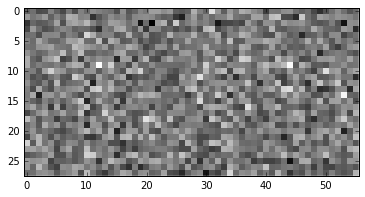
\includegraphics[scale=0.6]{learned_conv1_weights}
\caption{Visualisierung der gelernten Gewichter der ersten faltenden Schicht.}
\end{figure}
\begin{figure}[!h]
\centering
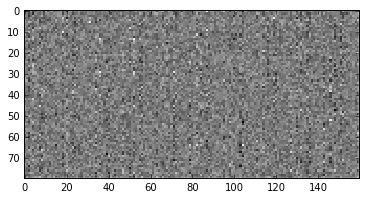
\includegraphics[scale=0.6]{learned_conv2_weights}
\caption{Visualisierung der gelernten Gewichter der ersten faltenden Schicht.}
\end{figure}

\noindent Dass das Netz tatsächlich inrgendwelche features erlernt hat, ist anhand der letzten beiden Abbildungen zu sehen. Faltet man eine homogene Bildfläche mit den gelernten Filtern, so entstehen linienartige Muster. Natürlich kann man keinen vierdimensionalen Tensor ohne manipulation darstellen, sodass wir diese auf zwei dimensionen umgeformt haben.

\begin{figure}[!h]
\centering
\includegraphics[scale=0.6]{conv1_on_plain_image}
\caption{Ausgabe der ersten faltenden Schicht für eine homogene Bildfläche.}
\end{figure}
\begin{figure}[!h]
\centering
\includegraphics[scale=0.8]{conv2_on_conv1_on_plain_image}
\caption{Ausgabe der zweiten faltenden Schicht.}
\end{figure}

\newpage
\section{Test und Auswertung}
Listing \ref{lst1}

\appendices
\newpage
\section{Code-Schnipsel}

\begin{lstlisting}[caption={Erzeugt ein Gewichts-Array mit zufällig initialisierten Werten. Die Dimensionen werden als Parameter entegengenommen.}, label=lst1]
def weight_variable(shape):
    """Creates a tf Variable of shape 'shape' with random elements"""
    initial = tf.truncated_normal(shape, stddev=0.1)
    return tf.Variable(initial)
\end{lstlisting}

\begin{lstlisting}[caption={Erzeugt ein bias-Array mit zufällig initialisierten Werten. Die Dimensionen werden als Parameter entegengenommen.}, label=lst2]
def bias_variable(shape):
    """Create a small bias of shape 'shape' with contants values of 0.1"""
    initial = tf.constant(0.1, shape=shape)
    return tf.Variable(initial)
\end{lstlisting}

\begin{lstlisting}[caption={Eine zweidimensionale Faltung mit Eingabe x und Filter W.}, label=lst3]
def conv2d(x, W):
    """Use a conv layer with weights W on zero padded input x and stride 1"""
    return tf.nn.conv2d(x, W, strides=[1, 1, 1, 1], padding='SAME')
\end{lstlisting}

\begin{lstlisting}[caption={Hier wird 2x2 max pooling auf die Eingabe x angewendet.}, label=lst4]
def max_pool_2x2(x):
    """Create a 2x2 pooling layer with strides 2, reducing the resolution"""
    return tf.nn.max_pool(x, ksize=[1, 2, 2, 1], strides=[1, 2, 2, 1], padding='SAME')
\end{lstlisting}

% Can use something like this to put references on a page
% by themselves when using endfloat and the captionsoff option.
\ifCLASSOPTIONcaptionsoff
  \newpage
\fi

\begin{thebibliography}{1}
\bibitem{vorlesung}
TODO: Namen einfügen, \emph{Vorlesung: Machine Learning II - Deep Learning}, WS 2016/17
\end{thebibliography}
\end{document}


